\subsubsection{21.11.14 (Соревнования)}

\begin{center}
	1-ый день соревнований "Робофест-Юг"
\end{center}
Сегодняшний день был посвящен тренировочным матчам.\newline

Внесенные доработки:
\begin{enumerate}
	\item Было обнаружено, что  робот теряет управления в случае попадания под колесо маленького (3 см) мяча. Для предотвращения таких ситуаций была установлена защита колес от мячей.
	
	\begin{figure}[H]
		\begin{minipage}[h]{0.2\linewidth}
			\center  
		\end{minipage}
		\begin{minipage}[h]{0.6\linewidth}
			\center{\includegraphics[scale=0.3]{days/21.11.14/images/01}}
			\caption{Защита от попадания мячей под колеса}
		\end{minipage}
	\end{figure}
	
	\item Нами было обнаружено, что основание подвижной корзины не заходит под днище робота, что не позволяет подвести ее как можно ближе к роботу. Для того, чтобы это исправить, было решено максимально увеличить клиренс задней части робота, повернув приводы в своих креплениях таким образом, чтобы вал привода располагался снизу. Это позволило увеличить расстояние между днищем и полом до 3,5 см, достаточных для прохождения основания подвижной корзины.
	
	\item Рейки, устанавливаемые на МЗК, были подрезаны до нужной длины и закреплены, однако из-за неисправности сервопривода, отвечающего за распирание реек, механизм захвата корзин был переделан. Неисправный сервопривод был демонтирован с захвата, а рейки были жестко закреплены.
	
	\begin{figure}[H]
		\begin{minipage}[h]{0.2\linewidth}
			\center  
		\end{minipage}
		\begin{minipage}[h]{0.6\linewidth}
			\center{\includegraphics[scale=0.3]{days/21.11.14/images/02}}
			\caption{Изменения в МЗК}
		\end{minipage}
	\end{figure}
	
	\item Был установлен Samanta-модуль и проведена одна тренировка на соревновательном поле.
	
	\begin{figure}[H]
		\begin{minipage}[h]{1\linewidth}
			\center{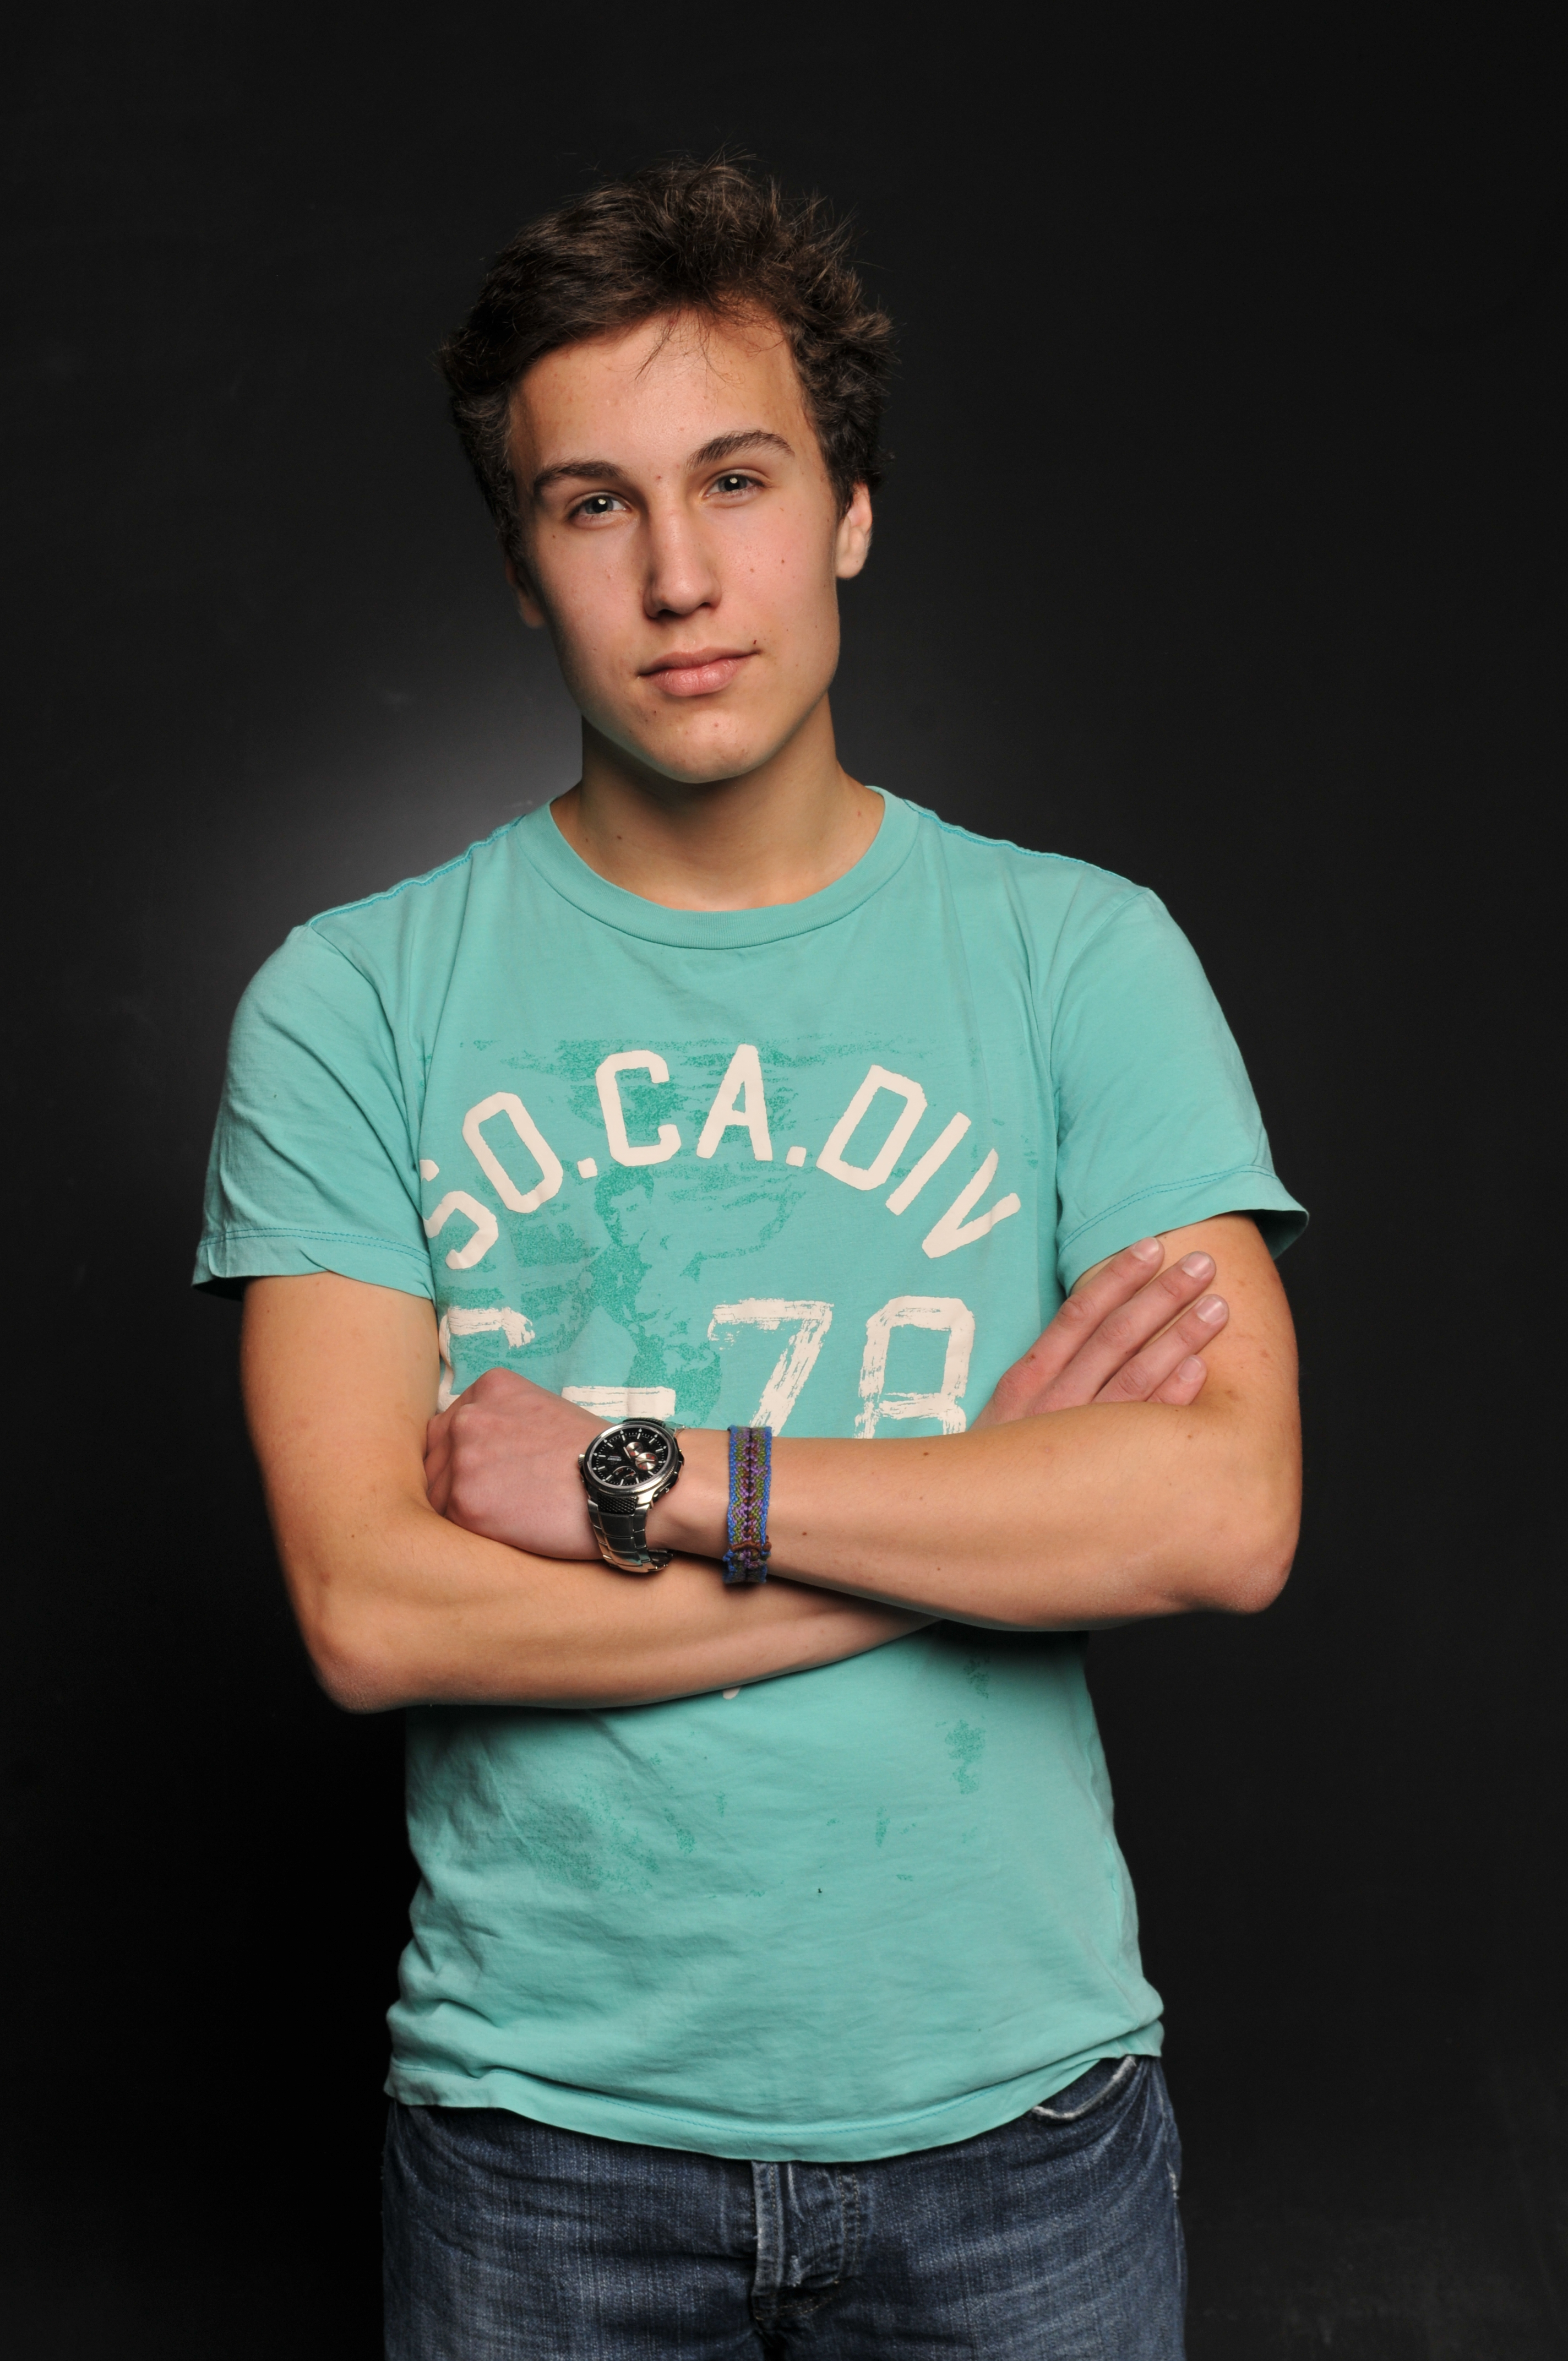
\includegraphics[scale=0.4]{days/21.11.14/images/03}}
		\end{minipage}
		\caption{Крепление Samanta}
	\end{figure}
	 	
\end{enumerate}
\fillpage